\documentclass[11pt,manuscript,screen,review]{acmart} % manuscript version
\usepackage{float, subcaption, graphicx, color, soul}
%% Rights management information.
\setcopyright{acmcopyright}
\copyrightyear{2021}
\acmYear{2021}

%% These commands are for a PROCEEDINGS abstract or paper.
% \acmConference[Conference acronym 'XX]{Make sure to enter the correct
%   conference title from your rights confirmation email}{June 03--05,
%   2018}{Woodstock, NY}

% \acmPrice{15.00}
% \acmISBN{978-1-4503-XXXX-X/18/06}

\begin{document}

\title{How to Git Gud: Skilled Gamers Optimize Interfaces for Performance}

%%
%% The "author" command and its associated commands are used to define
%% the authors and their affiliations.
%% Of note is the shared affiliation of the first two authors, and the
%% "authornote" and "authornotemark" commands
%% used to denote shared contribution to the research.
\author{Natalie Cottrill}
\email{natalie.cottrill@utah.edu}
\affiliation{%
  \institution{University of Utah}
  \city{Salt Lake City}
  \state{Utah}
  \country{USA}
}

\author{Jakob Johnson}
\email{jakob.johnson@utah.edu}
\affiliation{%
  \institution{University of Utah}
  \city{Salt Lake City}
  \state{Utah}
  \country{USA}
}

\author{Jessica Murdock}
\email{u0973401@utah.edu}
\affiliation{%
  \institution{University of Utah}
  \city{Salt Lake City}
  \state{Utah}
  \country{USA}
}

%%
%% The abstract is a short summary of the work to be presented in the
%% article.
\begin{abstract}
In competitive sports, human skill and performance, combined with high quality equipment and tools are deciding factors for success. In video gaming (esports), an optimized playing environment is essential. Keys to high performance include player skill, optimized software settings, and quality gear (including computers, monitors, audio input/output devices). In this study, we interviewed nine highly skilled esports players and surveyed 18 amateur players. We learn that both sets of players want high performance from their equipment and generally have high end hardware. We explore how expert players optimize their in-game software settings and team play performance. Our study also surveys ways that players prefer refining their gaming skills.
\end{abstract}

%%
%% Keywords
\keywords{esports, competitive gaming, video games, performance optimization, computer games, user experience, human-computer interaction}

\maketitle

\section{Introduction}
In-game settings can optimize performance and decrease latency in video game play \cite{Liu2021} which is typically demanding and requires a fast response. Display refresh rates, mouse, monitor, and GPU performance and settings all have important roles in maximizing a player's advantage in competitive gaming. Gameplay performance is critically important in esports, which is a billion-dollar industry \cite{ayles2019} with hundreds of millions of viewing hours and growing. 

Professional and high-level video game players push the limits of their gaming environment \cite{schell2018}. They are sensitive to minute changes in interfaces that affect recognition, speed, and recall, optimizing their software and hardware interfaces to maximize their performance. Video game players seek the most responsive and customizable equipment. Many video games, including those played in major esports, allow significant customization of game graphics and interface customization. Players tweak and change these settings to give them the best performance, either of their PC via graphics settings or of the player themselves through improved recognition speed or reaction time. Gamers push software and hardware developers to improve user interfaces to help their game play and are on the cutting edge of interface optimization. \cite{schell2018} We argue that HCI researchers can look to competitive video game players as an example group and use discoveries found in video games to advance the HCI field.

When competitors of similar skill challenge one another in tasks that depend on reaction time, the winner is generally the one who responds first. Hardware interfaces must respond quickly, display graphics as fast as possible, and offer low latency. When playing on teams, high level gaming performance also depends heavily upon efficient decision-making and communication. Esports games focus heavily on strategies and teamwork, allowing complex team play to overcome mechanical skill differences. Competitive esports games require almost constant communication from teammates, leadership, and decision-making skills to win. Developers create systems in the game to allow for responsive game play, displays, and effective communication. \cite{Alharthi2018}. 

In this paper, we seek to discover some of the ways that video game players optimize their gaming environment to improve their in-game performance. In order to capture a broad demographic group, we targeted expert video game players in semi-structured interviews as well as amateur players via an Amazon Mechanical Turk survey. 

\section{Background} % make sure to talk about related work here.
A number of prior studies examine how game performance is improved with better hardware. Better hardware decreases latency and increases graphics resolution and rendering. Researchers have observed that high refresh rates \cite{spjut2019} and low hardware latency are important factors in First Person Shooter games that require aim accuracy and speed. Their work shows that the time it takes to complete a gaming task gets worse as latency increases \cite{spjut2021}.

A cognitive study of gamers explored the habits of high performing players. Researchers found that those who played frequently, but in moderation and without long breaks, were able to gain skill the most efficiently. The best performers gained skill more rapidly when they habitually warmed up before game play with a regular routine. The study also found that habits developed during warm ups helped players when under pressure of the competition. \cite{huang2017}

Team dynamics and communication have also been identified as key to achieving optimal performance for esports players. Esports players need to communicate with teammates effectively and function well within the team. \cite{himmel2017} At least one study examined the performance of teams and studied how individuals improve their skills and learn how to work with others on a given shared mission. \cite{Sapienza2018}

Most prior research takes a fine-grained approach to study specific aspects of the gaming environment. Researchers have mostly analyzed hardware, software, and player performance as separate topics. Our research asks gamers about their playing background and preferences directly. We look at all of these aspects (hardware, individual and team performance) and pull them into a larger presentation of how players improve.

\subsection{Competitive Video Games}
Competitive video games are based upon players or teams of players playing against one another. In the end, one player or team wins and the other loses. These games have an explicit win or lose outcome. There are several popular competitive esports video games on the market that hit million dollar prize pools annually. In 2020, Counter Strike (CSGO) had the top prize pool of \$14.75M. \cite{murray2021} 

For example, in the tactical first-person shooter game VALORANT, a 5-player team must work together to plant a 'spike' on an objective, which another 5-player team defends. Each team must utilize unique hero character abilities to clear areas of the map and eliminate enemy players with a variety of guns. VALORANT is fairly new, releasing in 2020, but is quickly growing as an esports game. Other popular competitive multiplayer games include first person shooters Overwatch, Destiny 2, Apex Legends, and Call of Duty. Another popular genre is the multiplayer online battle arena (MOBA), with League of Legends and Dota 2 as the most popular titles.

\subsection{Gaming Equipment}
Gaming consoles like Switch, Xbox, and Playstation have long dominated the video game market. Recent improvements in personal computers (PCs) have inspired players to customize their home PCs and optimize them for gaming. \cite{hruska2020}

The participants we interviewed in this project were skilled gamers who regularly played competitive esports. Our participants primarily used PCs for their gaming experience. Of the expert competitive esports players, all played on PC, whereas among amateur players, 67\% played on PC. In this study, the hardware questions we asked of participants were primarily directed toward PCs. PCs can be customized to a player's preferences and our research focused upon how players optimize their game.

\section{Semi-Structured Interviews}

\subsection{Methodology}
We targeted high-level competitive first-person shooter players for our interviews. They have expert subject knowledge and play regularly. We approached the University of Utah (U of U) collegiate VALORANT team and the Florida Atlantic University (FAU) VALORANT team. Many players were interested in participating in the interview study, and we scheduled interview slots with nine different participants over several days. 

Interview participants ranged from 18 and 35 years old, with all but one of them between 18-21 years old. The interviews were conducted over voice communication platforms Discord \cite{discord} and Zoom \cite{zoom} and took roughly 30-45 minutes. 

We started with a slate of 26 questions that largely remained the same throughout the interview process. We made some minor changes in the interview questions follow-ups depending upon a participant’s responses. The interview style was informal and conversational to help the participants feel comfortable. The conversational style encouraged participants to talk about things that did not strictly relate to our questions. They would bring up other interesting insights and information that we would not have asked about and may not have been mentioned in a more formal interview style. Our questions fit into five categories; gaming background, playing environment, skills development, settings and hardware setup, and closing questions. 

After asking some basic demographic questions, we asked them about the video games they currently play, how frequently they play, and their skill level. These questions were designed to give us some background about the participant’s video game background and how much of an “expert” they might be. In the “playing environment” section, we asked questions about streaming online and watching streamers and professionals. We were also interested in how our participants usually play games; whether they played with a regular team or in “solo queue” - playing with teams formed by the game from random players.  

The following two sections were the bulk of the interview, diving deep into skills training and settings. We first asked questions about how the participants learned new skills or honed their existing skills and what attributes they felt were most important for competitive play. We asked the participant to share their in-game settings and explain why they chose them in the setup section. We then asked about their hardware setups, such as PC specs, monitor, mouse, and keyboard. 

In closing, we asked some open-ended questions about advice for players entering the competitive scene, as well as what they thought about the scene’s future. 

\subsection{Results}
\subsubsection{Participant Background and Gaming Practices}

All but one participant was currently enrolled in college, and all had some college education. Among the college majors, five of the nine participants had majors focused on computers: Computer Science, Game Design, or Information Systems.

On average, the participants spent about 20 to 25 hours a week playing video games. On the edges of this average, one participant played only 15 hours a week, while another participant reported spending 42-70 hours a week gaming. The latter participant was majoring in game design. 

Roughly more than 75\% of the participants’ overall gaming time was spent playing solely the competitive game they focus on, with the remaining time taken by various casual games. Most participants were in college or had day jobs, so most of their gameplay was in the evening after homework and work were finished. 

\subsubsection{Skills Training}

While some participants used aim training software to improve aim, it was not as prevalent as anticipated. The participants who used aim training software mostly used it as a game warmup or as a way to fine-tune their hardware settings. Participant five said “I think aim training or websites or like programs are only good at the start to like, get a feel for your mouse and the sensitivity. But then after, once in a while, or once you get used to it, [getting better is] more like practicing the in-game mechanics. So it's better to practice in-game at that point.” 

It was surprising that the competitive players we interviewed did not do extensive pregame warm-ups with aim training software or physical stretching or exercise. Of the competitive players who did do warm-up routines, they primarily consisted of jumping into a part of the game that was non-competitive to reawaken muscle memory and make sure they were ready to perform at peak levels.

While competitive players considered mechanical skills a basic need for good performance, almost all participants emphasized the importance of good communication. Many competitive video games are team-based and require participants to describe where they are and their situation (frequent and specific call-outs). A few participants noted that as team leads, they would choose a good communicator with average mechanical skills over a player who did not communicate with the team well but had perfect aim.

\subsubsection{Trends in Optimization}

Participants generally had specific and individualized software settings for dots per inch (DPI, a measure of mouse sensitivity within the mouse hardware), in-game mouse sensitivity, and cross-hair design. While at least one participant used 1500 DPI on their mouse, most players had used 400 or 800 DPI. One participant remarked, “At 400 [DPI], it is easier to move the mouse in a straight line, but you could miss a few pixels. At 800, it is harder to move in a straight line but it is easier to be more precise. You have to learn your own personal settings after starting with a good base.” 

Many participants scaled down their graphics settings and fidelity to increase frames-per-second (FPS). Some adjusted the colors enemies, and friendly players were outlined in, believing yellow outlines to be easier to see than red ones. Most of the participants had custom crosshair graphics, with some as small as a point comprising just a few pixels. Participants most often opted for a small four-rectangle crosshair, usually colored green, cyan, or red, to stand out from the background but not block their view. (Figure \ref{fig:crosshairs}). 

\begin{figure}[h]
    \centering
    \begin{subfigure}{0.3\linewidth}
        
\includegraphics[width=\linewidth]{img/tenz-cyan.png}
        \caption{Cyan crosshair}
    \end{subfigure}
    \begin{subfigure}{0.3\linewidth}
        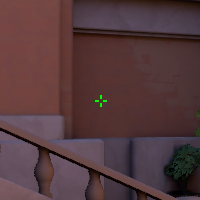
\includegraphics[width=\linewidth,]{img/tenz-green.png}
        \caption{Green crosshair}
    \end{subfigure}
    \begin{subfigure}{0.3\linewidth}
        
\includegraphics[width=\linewidth]{img/tiny.png}
        \caption{Small white crosshair}
    \end{subfigure}
    \caption{Examples of participant crosshairs}
    \label{fig:crosshairs}
\end{figure}

\subsubsection{Hardware}

We anticipated that most participants would focus on the mouse and mouse performance as the most critical hardware or that the graphics processing unit (GPU) would be at least as important as the mouse. However, most participants believed that monitors and their response and refresh rate were the most crucial piece of hardware for gameplay performance. Most participants had monitors with at least a 144 Hz refresh rate. It was notable that at least one participant had a monitor with a 360 Hz refresh rate. The participants who felt the monitor was most important noted that it was the piece of equipment that most boosted their reaction time.

While the monitor refresh rate was most often stated to be a key piece of equipment, several participants mentioned the weight and of the mouse as being important. Players generally favored very lightweight mice to reduce arm strain - a finding that we noted during a literature review\cite{Li2019}. In addition, of those players who gave mouse details, all used wireless devices and gave the reasoning that wired mice could cause surface tension or get tangled during gameplay. At least one player was so specific as to call out mouse data buffering as a spec that they considered purchasing a mouse.

\subsubsection{Closing Questions}

In the final open-ended questions, our participants shared their thoughts on the future of esports and offered advice to new players. All participants believed that the video game industry, in general, will continue to grow and that esports, in particular, would become more mainstream. Their general vision was that as today’s young players moved into other roles, like commentators or marketers, a new generation of competitive esports players would be coming into the sport, thus expanding the population of those familiar with esports. 

One of the most repeated words of advice to new players was, roughly paraphrased, “make sure to pick a game that you enjoy.” The usual motivation behind this advice was that even if a player lost a game, they could walk away having enjoyed it while thinking about what to do to improve.

\subsubsection{Summary}

In summary, we found that these experienced players practiced or played for many hours per week, from 20 to more than 50 hours. We found that many players had few warmup routines and preferred in-game play to practice drills. Their reasoning was that reminding their muscles of in-game mechanics was more important than just practicing aiming. The participants unanimously expressed that communication is the most critical skill in team-based games. Developers of video games and productivity software should be aware of this, allowing for quick and easy communication at all times so teamwork can flow smoothly. For performance, experienced gamers prioritize reaction time and precision, sometimes at the cost of visuals. They wanted control of the customization of details to find the setup that worked best for them, either graphical settings and colors or UI. Finally, players stressed the importance of liking the game, even in a defeat. Again developers and researchers should take note of this. Users working with a piece of software or playing a game for long periods should have an enjoyable experience despite their skill level. 

For hardware, the experts were in agreement that good hardware did make a significant impact on in-game player performance. They all used monitors with more than a 144 Hz refresh rate and the majority stated that it was the most important piece of hardware. Others mentioned the mouse as an important piece of hardware, noting specific aspects that helped them achieve better aim for longer. The experts used the best equipment they could afford, even if they knew it had reached the point of diminishing returns. In the case of their 360 Hz monitor, particpant four said "It's a little overkill, I regret buying it, don't buy it, it's not needed."  

\section{Online Questionnaire}

\subsection{Methodology}
To gain a more comprehensive view of how video game players optimize their gameplay, we broadened the field of participants to the broader audience of Amazon Mechanical Turk (AMT) workers. We published a survey consisting of questions similar to those we asked expert gamers. 

The survey was initially designed, maintained, and hosted on Qualtrics. To discourage bots, we required a randomly generated 3-digit code given to the user to be typed back in the form at the survey’s close. We also set parameters in Qualtrics to disallow an individual from taking the survey more than once. The questions we asked in the survey were modified versions of questions that we had asked our expert gamer participants. The questions were reworded to be approachable to a general audience. The Qualtrics survey was tested pre and post-publication for functionality and clarity.

The Qualtrics survey was then placed on Amazon Mechanical Turk (AMT) for presentation as a Human Interaction Task (HIT). For the survey’s title, we decided that the title “How Do You Play Video Games?” fit well and sounded compelling. The survey was not explicitly qualified. AMT offers pre-programmed demographic and topical fields that can be used to screen participants; none included video games or related topics. The amount of work and cost required to customize qualifications specific to persons who play video games was outside the scope of this research project. We attempted to use the survey’s description field to outline the survey requirements in anticipation that users would self-filter and only participate if they matched. Specifically, we asked AMT workers to take the survey only if they played video games for more than 1 hour a week. 

AMT’s default project settings were used to set up the survey for publication. Participants were offered \$1 for successful survey completion. With the resources allotted to this project, our survey was limited to 18 participants. While this is a small sampling relative to the large AMT user base, we decided that this number of people would provide sufficient data to compare their responses to those of the nine expert gamer participants we interviewed. We manually reviewed and approved questionnaires that seemed to include authentic responses. Only one submission was rejected because it was erroneous; the code in the submission was not in the range of codes we allotted.

\subsection{Results}

With only 18 responses, we cannot do rigorous statistical analysis on the results, but we can draw some conclusions from patterns in the data. We ended up rejecting one participant from AMT who entered an invalid survey code. We kept and paid out all other submissions.

First, in the demographics section, most of the participants are 25-34 years old and consider themselves experienced video gamers. Most played between 3-10 hours per week, with only a handful playing more than 10. 2/3 of the participants said they primarily play on a PC for gaming, with five on video game consoles and one primarily on their mobile phone (Figure \ref{fig:amt-platform}). They played a variety of games, with Call of Duty, Fortnite, and PlayerUnknown's Battlegrounds (PUBG) showing up the most.

\begin{figure}[h]
    \centering
    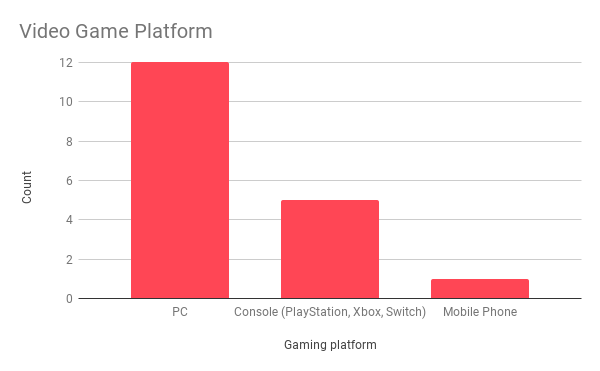
\includegraphics[width=0.5\textwidth]{img/amt-platform.png}
    \caption{Video Game Platform of survey respondents}
    \label{fig:amt-platform}
\end{figure}

When asked what they thought the most important skill required to win a game is, six said communication, and 7 said strategy, with only two prioritizing mechanical skill or aim. This result closely mirrors our expert interview, who agreed that communication with teammates was the most crucial skill to master. Eleven participants said they would look to video guides and tutorials to improve at a game, tying with watching professionals as the top ways to improve. 

All but one respondent said that the hardware setup was at least moderately important to a video gaming experience (Figure \ref{fig:amt-hardware}). 83\% preferred better performance (FPS or latency) over better visuals or graphics. Of the 12 PC players, only two had 60 Hz monitors, with the rest having 120 or 144 Hz monitors. These monitors are relatively new, showing how quickly they spread through the market. We included a question about the most important piece of hardware, with a variety of results. Two users mentioned playing racing simulator games and responded to this question, indicating their steering wheel as the most important, which we did not consider when developing the survey.

\begin{figure}[h]
    \centering
    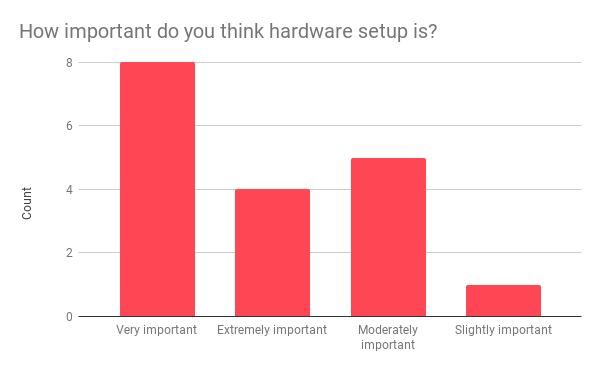
\includegraphics[width=0.5\textwidth]{img/amt-hardware.png}
    \caption{Hardware Importance}
    \label{fig:amt-hardware}
\end{figure}

% These stats are here just to help us flesh out the report on the hardware section.
%AMT = 67% PC, 28% console (switch, xbox, playstation), 5% mobile phone
%AMT = 67% said hardware very/extremely important
%AMT = 83% said they would adjust games for high performance and fast response over high quality graphics.
%AMT = Evenly split between gpu and monitor as most important hardware 33%
%AMT 67% high sensitivity
%AMT monitor refresh rate 83% 120Hz or more 17% 60 Hz.
%AMT 58% wireless mouse, 42% wired
%AMT intel 66%, i7 42%; AMD 34% Ryzen 5 17%
%AMT GPU nvidia 58%, amd 42 %

Finally, we asked about esports watching to gauge how connected to the pro scene the participants were. All but one participant said they at least occasionally watch esports (figure \ref{fig:amt-esports}), most watching Counter Strike: Global Offensive (CS:GO) or League of Legends. We asked an optional free-response question about how they thought the future of esports would be, and most felt that it would grow more in the future. With the majority watching esports, this response came as a surprise as it is still relatively small and not very popular. We suspect that the demographic of AMT users would probably not be representative of the general public, skewing towards young tech-savvy users who would more likely be interested in pro gaming. This result also reflects how frequently participants said they watch professionals to learn new skills in games.

\begin{figure}[h]
    \centering
    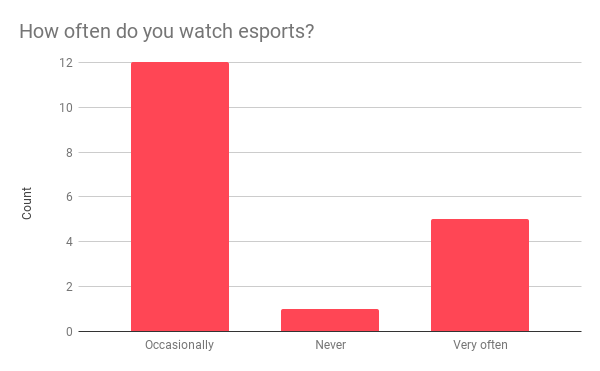
\includegraphics[width=0.5\textwidth]{img/amt-esports.png}
    \caption{Esports viewership of survey respondents}
    \label{fig:amt-esports}
\end{figure}

We also included a “bot check” question intended to filter out bot users or users who were not paying attention to the survey. Unfortunately, we tried to disguise the question too much, which made it somewhat confusing, and about a third of the users failed the question and opted to ignore it altogether. We would add an attention-check question that was more straightforward and impossible to misinterpret in the future. 

\section{Discussion}

In this study we examined the engaging esports gaming experience by identifying elements of the gaming environment and player skill that impact higher performance game play. Our research revealed many similarities between expert and amateur gamers. Both have closely related opinions regarding gaming hardware. Of all pieces of equipment, they valued a high refresh rate monitor the most. Likewise, they all preferred fast graphics response over high resolution graphics. Expert gamers tweaked internal game settings to minimize the depth and color range of graphics (set graphics to low) in order to increase frames per second (FPS). The equipment performance needs that our gaming participants shared with us match conclusions from hardware specialists. \cite{spjut2021} As esports continues to grow, so will the demand for high-speed graphics and interfaces that support exceptional player performance. 

Expert and amateur competitive players listed communication skills as one of the most important for a teammate to have. In fact esports requires rich and performant communication and collaboration tools, since teamwork is a core element. One company, Discord \cite{discord}, dominates the gaming industry in the communication tools arena. Software developers, especially communication and gaming UI specialists can study the reasons why gamers primarily using external communication tools.  

Both groups of players watch other professionals and online video guides as a primary means for improvement tips. A few expert gamers remarked that they would prefer to play with a teammate that has high communication skills and mediocre mechanical skills, instead of the other way around. 

Our research revealed several gaming aspects in which expert and amateur gamers differed. Expert gamers play nearly 3x more hours a week than amateur players. Some of our expert participants had specific practice hours where they played with their school's team, and others just played games whenever they are able. Surprisingly warmups among experts were fairly short, preferring to go right into gameplay. Since practicing mechanics in-game was mentioned as being more important than aim trainers developers should focus on making warmup modes that incorporate game mechanics in addition to aim training. 

Overall we learned a lot about the playing habits and optimization techniques of video game players. With esports growing rapidly, the HCI field should make sure to properly utilize and study it. We feel that the results of this research could lead to improvements in video games and beyond. 

\section{Limitations}

Despite the fact that we all attend a university with a lively esports community and several teams, it was still difficult to find and recruit expert players as participants. There aren't many official channels for communicating with esports players. We mostly found private Discord servers that we had to gain access to, and then attempt to interest some of the players present on them. Overall, we had difficulty gaining access to communication with esports players, and when we did, we only gained access to rather small pools to draw participants from.

Our research was also limited by how little time we had to conduct interviews. We spent less than a full week conducting all interviews, spending the week before on recruiting and the week after on transcribing and analyzing our results. Given more time, we could interview more players and perhaps gain a wider variety of answers and insights.

For our expert interviews we focused on players of one game - VALORANT - which though it is a major esports game, it represents only a small section of competitive games as a tactical first-person shooter. We were unable to interview players from other first-person shooter games or from other esports genres like MOBAs. This limits the scope and generalization of our research. It would be interesting to know what differences and similarities players of different genres have.

Due to our budget, our sample size for the AMT questionnaire was very small, and so our data may be skewed depending on those that participated.

It should be kept in mind that some of our participants were limited by budget in their hardware and software setup. Some pieces of equipment may appear more popular than they should, because they were a cheaper option for the participant, but not ideal for what they wanted.

Research on player game optimization, and high-performance interfaces of all kinds is sparse. It would have been helpful if we could have found more relevant information during our literature review before starting our own research.

\subsection{Future Work}

The list of game dynamics and environments in this study is not intended to be conclusive. Future research should expand the number of participants and the games they play, while also striving to include players from broader ranges of age, gender, and expertise. All of our participants were male and most were younger than 22 years.

Continuing this study, addressing the above limitations may open new possibilities for crafting more useful and intuitive tools and interfaces for esports players. In particular, better in-game collaboration tools and communication interfaces will enhance digital game development in this arena.

%% The acknowledgments section is defined using the "acks" environment
\begin{acks} 
    We acknowledge, with appreciation, the participation of members of the Owls Esports League, as well as the University of Utah and Florida Atlantic University Esports Leagues. We are grateful for the guidance of Eric Lang, John Lund, and Professor Tamara Denning. 
\end{acks}

%% The next two lines define the bibliography style to be used, and
%% the bibliography file.
\bibliographystyle{ACM-Reference-Format}
\bibliography{references}

\end{document}
\endinput
